%% LyX 2.3.6 created this file.  For more info, see http://www.lyx.org/.
%% Do not edit unless you really know what you are doing.
\documentclass[english]{article}
\usepackage[T1]{fontenc}
\usepackage[latin9]{inputenc}
\usepackage{babel}
\usepackage{float}
\usepackage{graphicx}
\usepackage[unicode=true,pdfusetitle,
 bookmarks=true,bookmarksnumbered=false,bookmarksopen=false,
 breaklinks=false,pdfborder={0 0 1},backref=false,colorlinks=false]
 {hyperref}

\makeatletter
%%%%%%%%%%%%%%%%%%%%%%%%%%%%%% User specified LaTeX commands.
\usepackage{geometry} % to change the page dimensions
\geometry{a4paper} % or letterpaper

\usepackage{graphicx} % support the \includegraphics command and options

\usepackage{amsmath} % for mathematical content
\usepackage{amsfonts} % for mathematical fonts

\usepackage{fancyhdr} % for better header layout
\pagestyle{fancy}
\usepackage{enumitem}
\usepackage{svg}

\makeatother

\begin{document}
\title{FreeRTOS Course}
\maketitle
\begin{center}

\includegraphics[scale=0.15]{/home/tonix/Documents/FreeRTOSCourse/Documentation/Presentations/CommonFigures/Universidad_Panamericana-logo}
\par\end{center}

\maketitle \tableofcontents \newpage

\section{Course Overview}

\subsection{Instructor Information}
\begin{center}
Name: Luis Emilio Tonix Gleason 
\par\end{center}

\begin{center}
Contact: ltonix@up.edu.mx
\par\end{center}

This course provides comprehensive training on FreeRTOS, targeting
embedded systems programmers who are looking to utilize the FreeRTOS
real-time operating system to its full potential in cricitcal system
where safety is a key role for a responsable project. Remeber safety
first.

\subsection{Prerequisites}

Participants are expected to have:

1. Basic knowledge of C programming

2. Microcontroller architectures.

3. Linux basics commands

4. Esp32 microcontroller

5. Windows/Linux Setup. MacOs not guarenteed to be supported

6. Git/Github: I will review your code and diagrams in this tool.
We can learn good coding standars and practices, and you will generate
a porfolio. 

\subsection{Assessment and Evaluation}

\begin{table}[h!] \centering \begin{tabular}{|l|c|} \hline \textbf{Assessment Component} & \textbf{Percentage} \\ \hline Class Participation & 10\% \\ \hline Homework Assignments & 20\% \\ \hline Midterm Examination & 20\% \\ \hline Project Design and Requirements First Delivery & 20\% \\ \hline Final Project Delivery & 30\% \\ \hline \end{tabular} \caption{Breakdown of assessment components and their corresponding weights in the course.} \label{table:assessment} \end{table}

Class participation involves responding to the professor's questions
on the topic currently being studied.

Some homework assignments are assessed through quizzes using the Kahoot
format.

Winners of the Kahoot quizzes receive additional bonus points that
can be used towards projects or exams.

\subsection{Objectives}
\begin{itemize}
\item Understand the core concepts of real-time operating systems. 
\item Learn how to configure,develop and run FreeRTOS on ESP32. 
\item Design and management of systems that must compute and provide results
within strict time constraints.
\item Designing and implementing effective emergency procedures and recovery
plans to handle potential disasters or failures.
\item Study of systems where failure could cause loss of life, significant
property damage, or environmental harm.
\end{itemize}

\section{Agenda}

\begin{enumerate}[label=\textbf{Week \arabic*:}]
 	\item \textbf{Introduction to Real-Time Systems}
    \begin{itemize}         
		\item What is an operating system?
		\item Main features of an OS
		\item Safety
		\item Security
		\item What is real time?     
		\item Introduction to Real-Time Operating Systems (RTOS) and their relevance in embedded solutions
		\item MIT License, GNU, MIT and GPL
		\item Understanding Copyleft
		\item Comparison of Open Sources Licenses
	\end{itemize}

	\item \textbf{Critical Systems and Applications of RTOS}     
	\begin{itemize}         
		\item Discussion of RTOS applications in critical systems across various industries:         
		\begin{itemize}             
		\item Aerospace and Aviation (e.g., General Electric, Hydra, DJI)             
		\item Automotive (e.g., Continental, NXP, Avnet)             
		\item Healthcare (e.g., Plexus, Baxter)             
		\item Power Generation (e.g., Baker Hughes, CERN)             
		\item Telecommunications (e.g., Cinvestav, Qualcomm)             
		\item Defense and Military (e.g., Hydra, A2E)         
		\end{itemize}     
	\end{itemize}

	\item \textbf{Good software practices (Part1)}

	\begin{itemize}         
		\item Overview of standard industry practices.         
		\item Importance of documentation and diagrams in maintaining scalable and maintainable code.
		\item Software Development Guide (SDG)
		\item Key components of an effective SDG.
		\item Software Detailed Document (SDD)  
		\item Requirments
		\item Exploring the role and structure of SDD.
		\item Unified Modeling Language (UML)
		\item Development process, good practices and coding standard
		\item Version control process GIT
		\item Test plan document 
		\item Whitebox testing and manual testing
		\item Understanding Continuous Integration 
		\item Benefits of integrating CI into the software development lifecycle.      	 
	\end{itemize}

	\item \textbf{Good software practices (Part2)}
	\begin{itemize}
		\item Practical perspective         
	\end{itemize}

	\item \textbf{FreeRTOS Architecture (Part 1)}      	
	\begin{itemize}          		
	\item Introduction to heap/stack memory management in RTOS.          		
	\item Detailed discussion on function pointers and the concept of callbacks.          		
	\item Overview of interrupt service routines and timer ISR.      	
	\end{itemize}

    \item \textbf{FreeRTOS Architecture (Part 2)}     
	\begin{itemize}         
		\item In-depth look at concurrent processing in FreeRTOS:         
		\begin{itemize}             
			\item Scheduler dynamics             
			\item Task management and priority settings             
			\item Queues, semaphores, and mutexes         
		\end{itemize}     
	\end{itemize}

    \item \textbf{Hands-on with ESP32 (Setup and Basic Examples)}     
	\begin{itemize}         
		\item Introduction to Espressif microcontrollers, with a focus on ESP32.         
		\item Setting up the development environment, including Visual Studio Code.         
		\item Configuring WSL for the Espressif FreeRTOS SDK.         
		\item Practical examples: Running basic GPIO LED control tasks.     
	\end{itemize}

    \item \textbf{Advanced Hands-on with ESP32}     
	\begin{itemize}               
		\item Techniques for effective serial debugging.
		\item WIFI drivers and code examples   
	\end{itemize}

	\item \textbf{Midterm Review and Examination}     
	\begin{itemize}         
		\item Review of all topics covered thus far.         
		\item Midterm examination to assess knowledge and practical application.     
	\end{itemize}
   

    \item \textbf{FreeRTOS Programming (Part 1)}     
	\begin{itemize}         
		\item Techniques for task creation and management.         
		\item Control functions such as delay, suspend, and resume.
		\item FreeRTOS configuration overview  
	\end{itemize}

	\item \textbf{FreeRTOS Programming (Part 2)}     
	\begin{itemize}         
		\item Comprehensive management of queues and semaphores.         
	\end{itemize}

	\item \textbf{Project Design, Requirements, UML and Planning for FreeRTOS Programming}     
	\begin{itemize}
	\item Detailed discussion on final project design and requirements.         
		\item Initial project planning and milestone setting.           
		\item Utilizing Unified Modeling Language (UML) to plan and model FreeRTOS projects.         
		\item Creating sequence diagrams and behavioral architectures for real-time systems.     
	\end{itemize}    

	\item \textbf{FreeRTOS Programming (Part 3)}
	\begin{itemize} 
		\item Detailed handling of software timers and event groups.
	\end{itemize}

	\item \textbf{IOT MQTT Programming}
	\begin{itemize} 
		\item MQTT introduction
		\item MQTT broker and subscriber
		\item hello world project MQTT with FreeRTOS
	\end{itemize}

    \item \textbf{Final Project workshop (Part 1)}     
	\begin{itemize}         
		\item Practical implementation of the final projects.         
		\item Final presentations and review sessions.     
	\end{itemize}

	\item \textbf{Final Project workshop (Part 2)}     
	\begin{itemize}         
		\item Practical implementation of the final projects.         
		\item Final presentations and review sessions.     
	\end{itemize}


\end{enumerate}

\newpage

\begin{figure}[H]
\begin{centering}
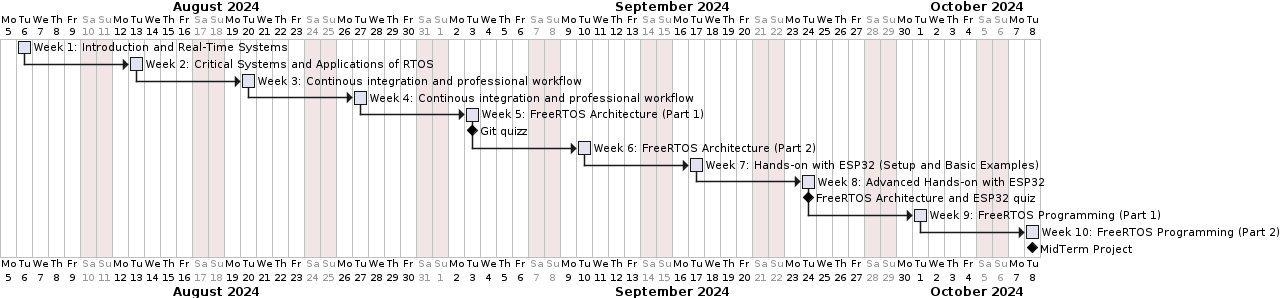
\includegraphics[scale=0.4]{PlanningPart1}
\par\end{centering}
\begin{centering}
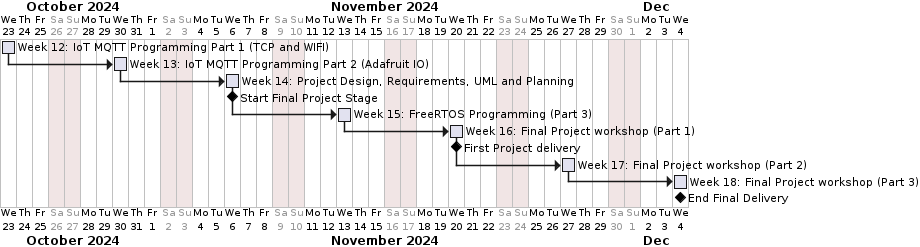
\includegraphics[scale=0.4]{PlanningPart2}
\par\end{centering}
\begin{centering}
\caption{Course Gannt}
\par\end{centering}
\end{figure}


\section{Course Content}

\subsection{Module 1: Introduction to Real-Time Systems}

\subsubsection{What exactly means Free?}

Overview of the implication of having an MIT license. What you should
and not do with this type of licence. 

\subsubsection{What is an Operating System?}

A generic overview of an operating sytem

\subsubsection{What is Real-Time?}

Diagrams to undertand the key concept of real time

\subsubsection{What does RTOS standfor?}

How RTOS are part for embbeded solutions 

\subsubsection{Critical systems}

Use cases for RTOS enviroments
\begin{itemize}
\item Aerospace and Aviation (General Electic) (Hydra) (Dji)
\item Automotive (Continental) (NXP) (Avnet) 
\item Healthcare (Plexus) (Baxter)
\item Power Generation (Baker Hughges)(Cern)
\item Telecommunications (Cinvestav)(Qualcomm)
\item Defense and Military (Hydra)(A2E)
\end{itemize}

\subsection{FreeRTOS Architecture}

\subsubsection{Basic Concepts}
\begin{itemize}
\item Heap/Stack Memory managment
\begin{itemize}
\item We need to know how this memory is managed because the RTOS task creating
will require to understand this
\end{itemize}
\item Function pointers
\begin{itemize}
\item Review of the callback concept
\end{itemize}
\item Interrupt service routine {[}Review{]}
\item Timer ISR
\end{itemize}

\subsubsection{Concurrent procesing in FreeRTOS}
\begin{itemize}
\item Scheduler
\item Task, priorities
\item Queues
\item Semaphores
\item Mutexes
\end{itemize}

\subsection{Hands on ESP32}

\subsubsection{Short story about spressif microcontrollers}

\subsubsection{Install visual studio code}

\subsubsection{WSL instalation for espressif FreeRTOS SDK}
\begin{itemize}
\item Download git FreeRTOS SDK project
\item Explore and open basic example
\item Configure COM ports to program
\item How to serial debug microcontroller
\item Run basic examples with GPIO LED
\end{itemize}

\subsection{How to do UML and planning for FreeRTOS programming}

\subsection{FreeRTOS Programming}

https://www.freertos.org/a00106.html
\begin{itemize}
\item Configuration 
\begin{itemize}
\item FreeRTOS configuration overview
\end{itemize}
\item Task Creation
\begin{itemize}
\item xTaskCreate vs xTaskCreateStatic
\item vTaskDelete
\item What task parameters mean?
\item Create one task that blink a led to high frequency
\item Create other task that blink a led with low frequency
\end{itemize}
\item Task Control
\begin{itemize}
\item vTaskDelay
\item vTaskDelayUntil
\item vTaskSuspend 
\item vTaskResume
\item xTaskResumeFromISR
\end{itemize}
\item Kernel Control
\begin{itemize}
\item vTaskStartScheduler
\item vTaskStepTick
\item vTaskStartScheduler
\end{itemize}
\item Task Utilities
\begin{itemize}
\item vTaskList
\item xTaskGetSchedulerState
\end{itemize}
\item Queue Management 
\begin{itemize}
\item xQueueCreate 
\item xQueueCreateStatic 
\item vQueueDelete 
\item xQueueSend 
\item xQueueSendFromISR
\item xQueueReceive 
\item xQueueReceiveFromISR
\end{itemize}
\item Semaphores 
\begin{itemize}
\item xSemaphoreCreateBinary 
\item xSemaphoreCreateBinaryStatic
\item xSemaphoreGive
\item xSemaphoreGiveFromISR
\end{itemize}
\item Software Timers
\begin{itemize}
\item xTimerCreate 
\item xTimerCreateStatic 
\item vTimerSetReloadMode 
\item xTimerStart 
\item xTimerStop 
\item xTimerChangePeriod 
\item xTimerDelete 
\item xTimerReset 
\end{itemize}
\item Event Groups 
\begin{itemize}
\item vEventGroupDelete 
\item xEventGroupClearBits 
\item xEventGroupClearBitsFromISR 
\item xEventGroupCreate 
\item xEventGroupCreateStatic 
\item xEventGroupGetBits 
\item xEventGroupGetBitsFromISR 
\item xEventGroupGetStaticBuffer 
\item xEventGroupSetBits 
\item xEventGroupSetBitsFromISR 
\end{itemize}
\end{itemize}

\section{Final project }

For a final project in a FreeRTOS class that involves the implementation
of a critical system, you could consider designing a \textquotedbl Smart
Emergency Response System.\textquotedbl{} This project would integrate
various sensors, communication modules, and control outputs to create
a comprehensive emergency management system suitable for environments
like industrial facilities, schools, or public buildings. The SERS
will use FreeRTOS to manage the concurrent operations of various sensors
and actuators to detect and respond to emergencies such as fires,
gas leaks, and unauthorized access. The system will prioritize tasks
based on the severity and type of emergency, ensuring that the most
critical responses are handled first.

\subsection{Software Requirements:}
\begin{enumerate}
\item Design
\begin{enumerate}
\item Software squence diagram, representing task comunication
\item Behavioral architecture
\item Software Detail Design Document and the critical constrains to be
met. 
\end{enumerate}
\item FreeRTOS Configuration: 
\begin{enumerate}
\item Implement tasks
\item Queues
\item Semaphores
\item Mutexes.
\end{enumerate}
\item Task Scheduling:
\begin{enumerate}
\item High priority tasks for immediate threats (e.g., fire detection and
response). 
\item Lower priority tasks for non-immediate alerts (e.g., unauthorized
access).
\end{enumerate}
\item Interrupt Service Routines (ISR): For immediate processing of critical
sensor data.
\item Communication Protocol: Implementation for sending real-time data
and alerts.
\end{enumerate}

\section{Materials and Resources}

https://www.freertos.org/Documentation/Mastering-the-FreeRTOS-Real-Time-Kernel.v1.0.pdf
\end{document}
